% Jake's final-data section and Word replacement blocks, 14 October 2026.
% Compile from this directory, e.g. pdflatex "jakes section.tex" (twice).
% Main text ends at the explicit MAIN SECTION END marker below.
% Subsequent pages contain Appendix D, references and labelled Word replacement blocks.
% Figures: .venv/bin/python scripts/build_jakes_figures.py from the project root.
% Data and saved model outputs are unchanged. HAR_QTFE and Tim_VAR are untouched.
\documentclass[11pt,a4paper]{article}
\usepackage[margin=1in]{geometry}
\usepackage[T1]{fontenc}
\usepackage{newtxtext,newtxmath}
\usepackage{amsmath,booktabs,array,tabularx,graphicx,float,caption}
\usepackage[round,authoryear]{natbib}
\usepackage[hidelinks]{hyperref}
\usepackage{microtype}
\graphicspath{{jakes_figures/}{latex_report/jakes_figures/}}
\setlength{\parindent}{0pt}
\setlength{\parskip}{5pt}
\setlength{\tabcolsep}{5pt}
\renewcommand{\arraystretch}{1.12}
\captionsetup{font=small,labelfont=bf,justification=raggedright,singlelinecheck=false}
\hypersetup{pdftitle={Jake's section: leverage-augmented VAR},pdfauthor={Jake Lockitch}}
\newcommand{\reportnote}[1]{\par\smallskip{\footnotesize\raggedright #1\par}}
\begin{document}

% ==================== MAIN SECTION START ====================
\section*{3.3 Leverage-augmented VAR (LVAR)}

Realised variance measures how much prices move, but does not show whether the market ends higher or lower. Two days can have similar variance even if equity prices rise on one and fall on the other. We therefore ask whether recent equity price falls help predict future equity variance. We add three measures of negative ES returns to a standard VAR and call this the \emph{leverage-augmented VAR} (LVAR). We then test whether commodity information adds further value.

The model uses past variances and the three return measures to predict variance at the next observation in the common panel:
\begin{equation}\label{eq:jake-lvar}
 z_{t+1}=c+\sum_{j=1}^{p} A_jz_{t+1-j}+\Gamma d_t+u_{t+1},
 \qquad p=5.
\end{equation}
Here, $z_t$ contains ES log RV5 and the log variances of the included commodities. The matrices $A_j$ give the weights on the previous five variance observations, while $\Gamma$ gives the weights on the three return measures in $d_t$. The constant is $c$, and $u_{t+1}$ is the part the model does not explain. We estimate the weights by ordinary least squares (OLS), separately for each market equation, following the standard VAR framework \citep{lutkepohl}. The weights are learned from the data: a negative return does not automatically raise the variance forecast.

The leverage effect describes the tendency for negative equity returns to be associated with higher future variance. Following the idea of persistent leverage in \citet{corsi-reno}, we measure negative ES returns over the previous 1, 5 and 22 observations. For decimal close-to-close log returns $r_t$, these measures are
\begin{equation}\label{eq:jake-downside}
 d_t=(d_t^{(1)},d_t^{(5)},d_t^{(22)})',\qquad
 d_t^{(h)}=\left|\min\left(\frac{1}{h}\sum_{i=0}^{h-1}r_{t-i},0\right)\right|.
\end{equation}
Each measure is zero when the average return is positive or zero. When the average is negative, we use its magnitude. For example, an ES return of $-2\%$ gives a daily measure of $0.02$, while a return of $+2\%$ gives zero. The supplied percentage returns are divided by 100. For the 5- and 22-observation measures, we first average the signed returns, allowing gains and losses to offset each other, and then measure the size of a negative average. These three leverage inputs are also called \emph{downside controls}. They enter every equation and use only returns observed before the forecast target.

To measure what the return information adds, we compare LVAR with a plain VAR that uses the same variance lags, training observations and forecast dates. The plain VAR leaves out $\Gamma d_t$. We also compare models with commodities against an equity-only LVAR that keeps the same return measures. This separates the benefit of negative-return information from the benefit of adding commodities. We label the equity-only versions VAR and LVAR for consistency; with only one variance series, they are mathematically autoregressions. Unlike the VAR in Section 3.2, these models have no Treasury or calendar controls and use five rather than four variance lags. We therefore use our own plain benchmark to measure the leverage contribution.

We use the final dataset described in Section 2. Building the lagged variables and return averages leaves 3,867 estimation outcomes, including 3,084 initial training outcomes through 12 July 2023. BIC on the training-only five-market plain VAR selects five lags from candidates 1--20; each candidate uses the same outcomes. We keep five lags for all main VAR and LVAR comparisons. AIC selects ten, which we examine separately. The 1/5/22 return windows are fixed, as in LHAR, rather than selected by BIC.

We produce 783 forecasts from 13 July 2023 to 31 August 2026. Before each forecast, the model is fitted using only observations available at that point. Once the next outcome is observed, it is added to the training history for later forecasts. This expanding procedure never uses future commodity values or future equity returns.

\setcounter{table}{1}
\begin{table}[H]
\centering\small
\caption{Out-of-sample accuracy of selected VAR and LVAR specifications}
\label{tab:jake-results}
\begin{tabular}{@{}p{8.1cm}rrr@{}}\toprule
Model & ES coefficients & MSE & MAE\\\midrule
Equity-only VAR(5) & 6 & 0.368531 & 0.464175\\
Equity-only LVAR(5) & 9 & 0.334215 & 0.442837\\
LVAR: oil and gold & 19 & 0.336611 & 0.443919\\
LVAR: natural gas & 14 & 0.332670 & 0.442343\\
LVAR: oil, natural gas and gold & 24 & 0.334549 & 0.443412\\
LVAR: all four commodities & 29 & 0.334687 & 0.443561\\\bottomrule
\end{tabular}
\reportnote{Notes: all models forecast the same 783 ES log-RV5 outcomes from 13 July 2023 to 31 August 2026, using five variance lags and an expanding estimation sample. Every LVAR adds the same three leverage inputs (downside controls). Lower MSE and MAE indicate smaller errors. Coefficient counts include the intercept and refer to the ES equation. ``All four'' means oil, corn, gold and natural gas. Source: own calculations in \texttt{VAR\_QTFE.ipynb}, final-data run of 13 October 2026.}
\end{table}

Adding the three leverage inputs to the equity-only VAR(5) lowers MSE from 0.368531 to 0.334215, an improvement of 9.31\%. The return measures therefore provide useful forecast information beyond past equity variance in this comparison. Adding oil and gold to the equity-only LVAR raises MSE by 0.72\%, and adding all four commodities raises it by 0.14\%. Natural gas alone lowers MSE by 0.46\%. These commodity differences are small. The descriptive uncertainty intervals in Table~\ref{tab:jake-intervals} include zero for the commodity comparisons, while the leverage improvement remains positive across the checks. We find a clearer benefit from equity-return information than from additional commodities.

Joint coefficient tests in Table~\ref{tab:jake-joint-tests} show that some commodity histories help explain the observations used to estimate the model. This does not mean they improve forecasts of later observations. The results do not establish that commodities and equities are unrelated; they show limited additional forecasting value in these models and over this evaluation period. Conditional commodity-to-equity impulse responses are reported in Figure~\ref{fig:jake-irfs} in Appendix D.

There are also reasons to interpret the results cautiously. ADF and KPSS give conflicting evidence about stationarity. The estimated VAR dynamics pass the stability check, but the residuals still show dependence over time, so the model does not capture every pattern in the data. We use standard errors that allow for autocorrelation and changes in error variance (HAC with bandwidth 22; \citealp{newey-west}). This adjusts the reported uncertainty, but does not solve the stationarity issue or missing model dynamics. With ten lags, the equity-only model with downside controls has MSE 0.328510, and adding oil and gold still does not improve its forecast accuracy. Because the evaluation period has already been examined, these findings remain exploratory. We do not test causal effects or whether the forecasts improve portfolio or risk-management decisions.
% ==================== MAIN SECTION END ====================

\clearpage
% ==================== APPENDIX D START ====================
\section*{Appendix D: LVAR specification and checks}
\setcounter{table}{0}
\setcounter{figure}{0}
\renewcommand{\thetable}{D\arabic{table}}
\renewcommand{\thefigure}{D\arabic{figure}}

This appendix supports the LVAR in Section 3.3. The main specification uses five variance lags, an intercept and the downside measures in Equation~\eqref{eq:jake-downside}, without Treasury or calendar controls. Forecasts use the same 783 evaluation targets as Section 3.2, from 13 July 2023 to 31 August 2026. Appendix B covers Section 3.2's different VAR specification.

\subsection*{D.1 Lag selection and forecast sensitivity}

AIC and BIC use the plain five-market system (equity, oil, corn, gold and natural gas), estimated only on the initial training sample through 12 July 2023. Each candidate uses the same 3,084 outcomes. BIC selects five variance lags; AIC selects ten. The downside windows stay fixed at 1, 5 and 22 observations.

\begin{figure}[H]
\centering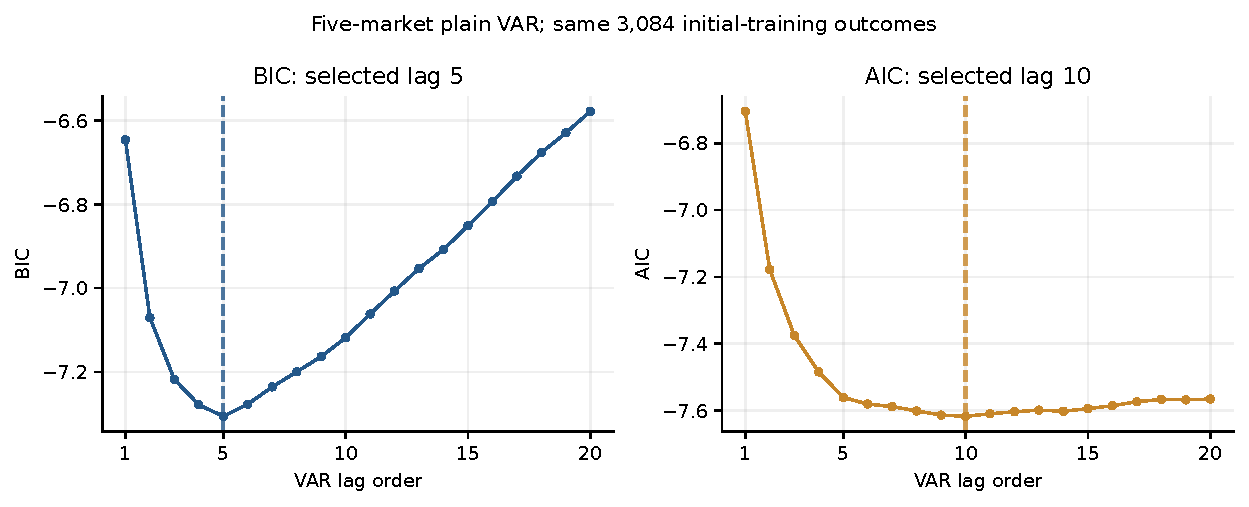
\includegraphics[width=\linewidth]{lag_selection.pdf}
\caption{Lag selection for the initial-training five-market VAR}
\label{fig:jake-lags}
\reportnote{Notes: the system includes an intercept and variance lags, without downside, Treasury or calendar controls. Each candidate uses the same training outcomes. Source: own calculations.}
\end{figure}

\begin{table}[H]
\centering\small
\caption{Forecast accuracy with five and ten variance lags}
\label{tab:jake-lag-sensitivity}
\begin{tabularx}{\linewidth}{@{}Xrrrr@{}}\toprule
& \multicolumn{2}{c}{MSE} & \multicolumn{2}{c}{MAE}\\
Model & 5 lags & 10 lags & 5 lags & 10 lags\\\midrule
Equity-only VAR & 0.368531 & 0.365940 & 0.464175 & 0.463306\\
Equity-only LVAR & 0.334215 & 0.328510 & 0.442837 & 0.440629\\
LVAR: oil and gold & 0.336611 & 0.330827 & 0.443919 & 0.442912\\
LVAR: natural gas & 0.332670 & 0.328684 & 0.442343 & 0.441537\\
LVAR: oil, natural gas and gold & 0.334549 & 0.330157 & 0.443412 & 0.442896\\
LVAR: all four commodities & 0.334687 & 0.330471 & 0.443561 & 0.442872\\
\bottomrule\end{tabularx}
\reportnote{Notes: 783 common forecast targets and an expanding estimation sample. Lower values indicate smaller errors. Equity-only VAR and LVAR are single-variable autoregressions; every LVAR includes the same three leverage inputs. ``All four'' means oil, corn, gold and natural gas. Source: own calculations.}
\end{table}

Downside controls reduce equity-only MSE by 9.31\% at five lags and 10.23\% at ten lags. At ten lags, every reported commodity extension has higher MSE than the equity-only model with downside controls. The small natural-gas advantage at five lags therefore does not persist in this check.

\clearpage
\subsection*{D.2 Stationarity and fitted-model checks}

\begin{table}[H]
\centering\small
\caption{Stationarity tests for the initial-training log-RV5 series}
\label{tab:jake-stationarity}
\begin{tabularx}{\linewidth}{@{}Xrrrr@{}}\toprule
Series & ADF statistic & ADF $p$ & KPSS statistic & KPSS $p$\\\midrule
Equity & -5.5373 & $<0.001$ & 0.8349 & $\leq 0.010$\\
WTI oil & -3.9928 & 0.0014 & 1.9409 & $\leq 0.010$\\
Gold & -5.1617 & $<0.001$ & 0.9606 & $\leq 0.010$\\
Natural gas & -3.9078 & 0.0020 & 2.6295 & $\leq 0.010$\\
Corn & -5.5897 & $<0.001$ & 0.8136 & $\leq 0.010$\\
\bottomrule\end{tabularx}
\reportnote{Notes: 3,106 observations per series, from 3 February 2011 to 12 July 2023. Both tests include an intercept and no trend. ADF selects its auxiliary lags by AIC; KPSS uses an automatic bandwidth. KPSS probabilities are bounded by its lookup table; values of 0.010 indicate $p\leq0.010$. Probabilities below 0.001 are displayed as $<0.001$. Source: own calculations.}
\end{table}

ADF rejects a unit root for every series, while KPSS rejects level stationarity. This conflicting evidence prevents an unqualified claim that the series are stationary. The fitted-model checks below assess stability and unexplained patterns separately.

\begin{table}[H]
\centering\small
\caption{Initial-training stability and equity-residual checks for LVAR(5)}
\label{tab:jake-diagnostics}
\begin{tabularx}{\linewidth}{@{}Xrrr@{}}\toprule
Model & Largest root & Ljung--Box $p$ & ARCH $p$\\\midrule
Equity-only LVAR & 0.9159 & $<0.001$ & 0.4184\\
LVAR: oil and gold & 0.9669 & $<0.001$ & 0.3726\\
LVAR: oil, natural gas and gold & 0.9777 & 0.0018 & 0.3227\\
LVAR: all four commodities & 0.9786 & 0.0019 & 0.3126\\
\bottomrule\end{tabularx}
\reportnote{Notes: 3,084 training outcomes. The largest root is the modulus of a companion-matrix eigenvalue, conditional on the downside controls. Values below one satisfy the variance-dynamics stability condition. Ljung--Box tests use 30 residual lags without a fitted-parameter degrees-of-freedom adjustment; ARCH tests use five lags. These are diagnostic checks. Source: own calculations.}
\end{table}

The reported roots are below one, but the Ljung--Box results indicate remaining residual dependence. The ARCH tests do not reject their null at 5\%. Passing these stability or ARCH checks does not establish stationarity or complete model adequacy.

\begin{table}[H]
\centering\small
\caption{Joint tests of commodity-lag coefficients in the equity equation}
\label{tab:jake-joint-tests}
\begin{tabularx}{\linewidth}{@{}Xrrr@{}}\toprule
Model & Coefficients tested & Wald statistic & HAC $p$\\\midrule
LVAR: oil and gold & 10 & 37.7788 & $<0.001$\\
LVAR: oil, natural gas and gold & 15 & 63.7299 & $<0.001$\\
LVAR: all four commodities & 20 & 69.6887 & $<0.001$\\
\bottomrule\end{tabularx}
\reportnote{Notes: the null sets all included commodity-lag coefficients in the equity equation to zero, conditional on equity lags and downside controls. Tests use 3,084 initial-training outcomes and HAC covariance with bandwidth 22. Reported probabilities use an asymptotic chi-squared reference distribution. Source: own calculations.}
\end{table}

The joint tests indicate in-sample predictive information from the commodity histories. Mixed stationarity evidence and remaining residual dependence warrant caution with inference. These results do not establish causal effects or improvements in out-of-sample forecasting.

\clearpage
\subsection*{D.3 Uncertainty around forecast improvements}

Figure~\ref{fig:jake-gains} and Table~\ref{tab:jake-intervals} compare each candidate with its named benchmark on the same forecast dates. Positive gains indicate lower MSE for the candidate. To describe uncertainty, we resample the paired forecast losses in circular blocks of 20 observations, using 2,000 draws. Resampling blocks keeps some dependence between nearby observations. The intervals are descriptive and are not formal nested-model or selection-adjusted significance tests.

\begin{figure}[H]
\centering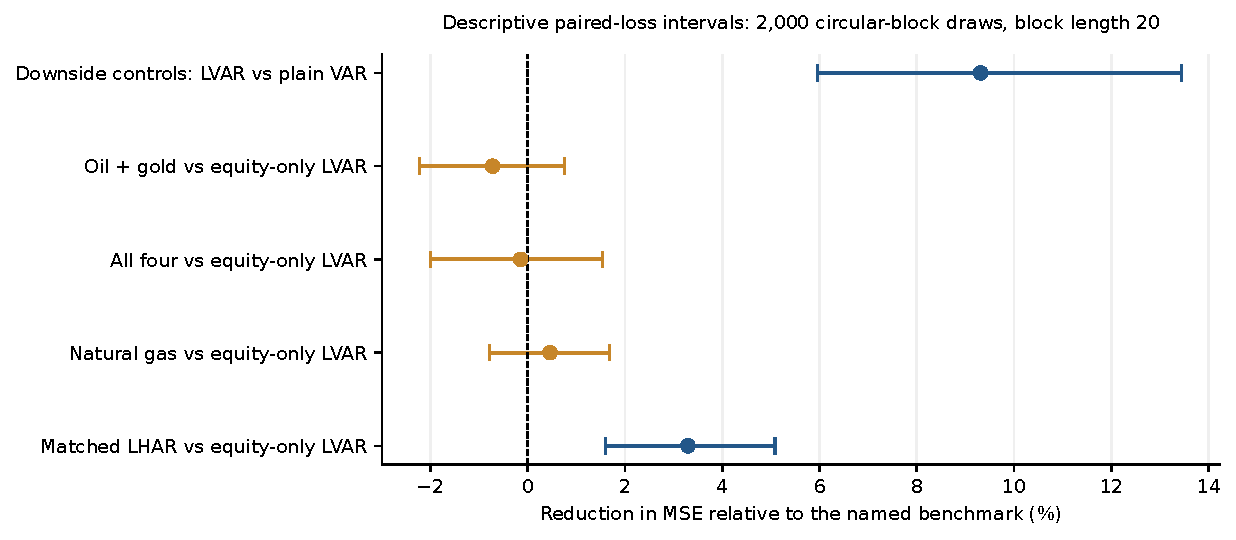
\includegraphics[width=\linewidth]{incremental_gains.pdf}
\caption{Incremental forecasting value of downside controls and commodities}
\label{fig:jake-gains}
\reportnote{Notes: points show percentage reductions in MSE relative to the named benchmark. Bars are descriptive 95\% paired-loss intervals; the dashed line marks zero gain. The LHAR comparison is recomputed on the same 783 targets and differs from the original HAR notebook's separate 80/20 split. Source: own calculations.}
\end{figure}

\begin{table}[H]
\centering\small
\caption{MSE reductions and descriptive uncertainty intervals}
\label{tab:jake-intervals}
\begin{tabularx}{\linewidth}{@{}X*{3}{>{\raggedleft\arraybackslash}p{1.75cm}}@{}}\toprule
Comparison & Gain (\%) & Lower (\%) & Upper (\%)\\\midrule
Equity-only LVAR vs equity-only VAR & 9.31 & 5.95 & 13.44\\
Oil and gold vs equity-only LVAR & -0.72 & -2.21 & 0.77\\
All four commodities vs equity-only LVAR & -0.14 & -2.00 & 1.55\\
Natural gas vs equity-only LVAR & 0.46 & -0.79 & 1.69\\
Matched equity-only LHAR vs equity-only LVAR & 3.30 & 1.59 & 5.09\\
\bottomrule\end{tabularx}
\reportnote{Notes: all models use five variance lags, except LHAR, which uses fixed 1/5/22 variance averages. The gain is $100(1-\mathrm{MSE}_{\mathrm{candidate}}/\mathrm{MSE}_{\mathrm{benchmark}})$. Bounds are the 2.5th and 97.5th percentiles from 2,000 circular-block draws with block length 20. Negative gains indicate higher MSE. Source: own calculations.}
\end{table}

The leverage-input interval is entirely positive, while each commodity interval includes zero. The leverage interval also remains positive when block lengths of 5 and 60 are used. The common-date LHAR comparison shows a descriptive advantage over the equity-only LVAR. Together, these checks provide clearer evidence of forecasting value from equity-return information than from additional commodities in the reported specifications. Because the evaluation period has already been examined, the findings remain exploratory and do not establish general model superiority or benefits for portfolio and risk-management decisions.

\clearpage
\subsection*{D.4 Conditional commodity-to-equity impulse responses}

We examine how the fitted all-four-commodity LVAR(5) responds to an innovation in each commodity's log realised variance, following the generalised impulse-response approach of \citet{pesaran-shin}. The model is estimated on the initial 3,084 training outcomes through 12 July 2023. We compare a shocked system with a baseline system that has the same path for the predetermined equity-return controls. These responses therefore describe the variance dynamics conditional on those controls.

\begin{figure}[H]
\centering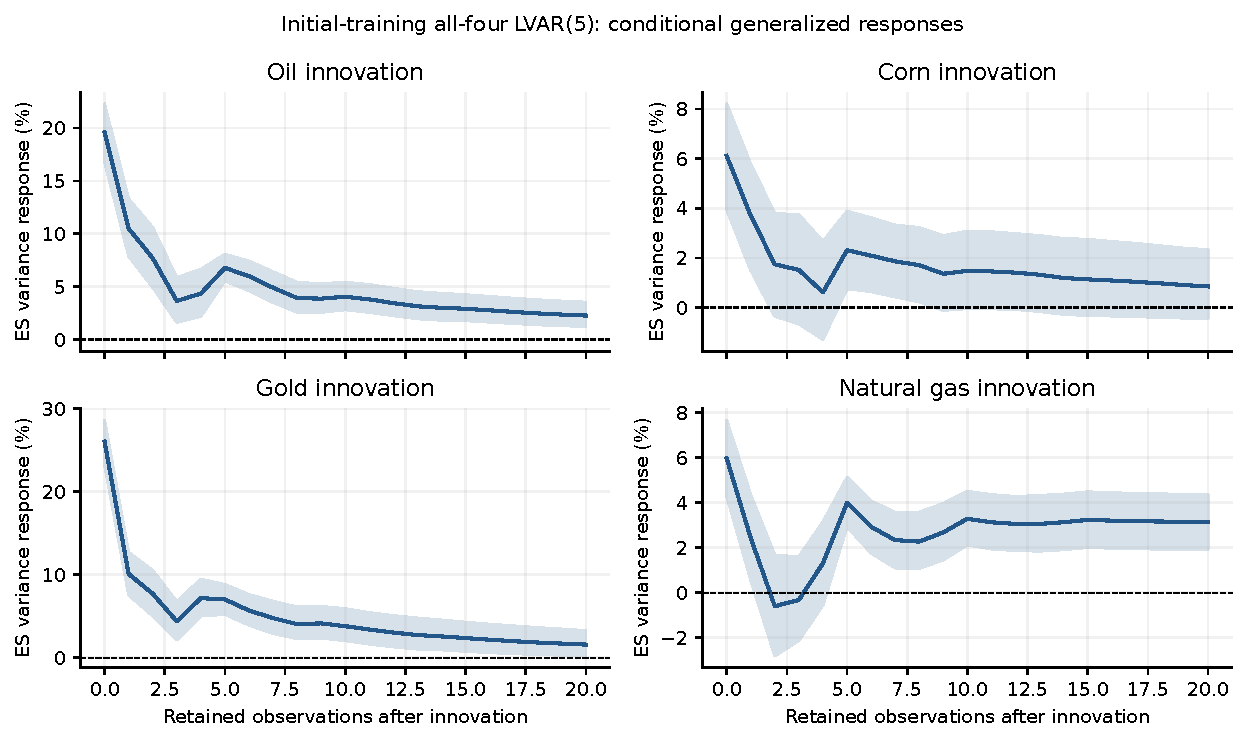
\includegraphics[width=\linewidth]{conditional_irfs.pdf}
\caption{Conditional commodity-to-equity impulse responses in the initial-training LVAR(5)}
\label{fig:jake-irfs}
\reportnote{Notes: each shock is one residual standard deviation of commodity log RV5, allowing contemporaneously correlated innovations. Responses show percentage changes in ES variance over 0--20 retained observations. The shocked and baseline systems have identical downside-control paths. Shading gives exploratory 95\% pointwise bands from 2,000 joint-HAC normal parameter simulations with bandwidth 22. These are not simultaneous bands or forecast prediction intervals. Source: own calculations, notebook Section 8.}
\end{figure}

Oil and gold have larger immediate estimated ES variance responses than corn and natural gas. The oil and gold responses generally decline over the horizon, while the natural-gas response remains positive at observation 20. Shock sizes differ across commodities because each uses its own residual standard deviation. The response at observation zero includes contemporaneous co-movement. These curves describe estimated relationships within the fitted system; they do not identify causal effects or establish that commodity inputs improve forecast accuracy.
% ==================== APPENDIX D END ====================

\clearpage
\begin{thebibliography}{9}
\bibitem[Corsi and Ren\`o(2012)]{corsi-reno}
Corsi, F., and Ren\`o, R. (2012). Discrete-time volatility forecasting with persistent leverage effect and the link with continuous-time volatility modeling. \emph{Journal of Business \& Economic Statistics}, 30(3), 368--380. \href{https://doi.org/10.1080/07350015.2012.663261}{doi:10.1080/07350015.2012.663261}.

\bibitem[L\"utkepohl(2005)]{lutkepohl}
L\"utkepohl, H. (2005). \emph{New Introduction to Multiple Time Series Analysis}. Springer. Chapters 2--4 on stable VAR processes, estimation, order selection and model adequacy. \href{https://doi.org/10.1007/978-3-540-27752-1}{doi:10.1007/978-3-540-27752-1}.

\bibitem[Newey and West(1987)]{newey-west}
Newey, W.~K., and West, K.~D. (1987). A simple, positive semi-definite, heteroskedasticity and autocorrelation consistent covariance matrix. \emph{Econometrica}, 55(3), 703--708. \href{https://doi.org/10.2307/1913610}{doi:10.2307/1913610}.


\bibitem[Pesaran and Shin(1998)]{pesaran-shin}
Pesaran, M.~H., and Shin, Y. (1998). Generalized impulse response analysis in linear multivariate models. \emph{Economics Letters}, 58(1), 17--29. \href{https://doi.org/10.1016/S0165-1765(97)00214-0}{doi:10.1016/S0165-1765(97)00214-0}.

\end{thebibliography}

\clearpage
% ==================== WORD REPLACEMENTS START ====================
\renewcommand{\thetable}{\arabic{table}}
\section*{Word block A: Section 4, Empirical results}

\textbf{Destination and action (do not paste this instruction):} replace the entire square-bracketed paragraph beginning ``[Leveraged VAR results to be added'' with the two paragraphs and Table 4 below. Keep the existing HAR and Section 3.2 VAR results.

The leverage-augmented VAR is compared with its own plain VAR benchmark, using the same five variance lags, commodity sets and 783 forecast dates. Adding the three negative-return measures reduces equity-only MSE from 0.368531 to 0.334215, an improvement of 9.31\%. Table 4 shows that the reported LVAR specifications also outperform the corresponding plain VARs with the same commodities. This comparison isolates the contribution of the leverage inputs within the Section 3.3 specification, rather than comparing it with Section 3.2's differently specified VAR.

Commodity information adds little once the leverage inputs are included. Relative to the equity-only LVAR, oil and gold raise MSE by 0.72\%, all four commodities raise it by 0.14\%, and natural gas alone lowers it by 0.46\%. The descriptive uncertainty intervals for these commodity comparisons include zero (Table D5). At ten lags, none of the reported commodity extensions improves on the equity-only LVAR (Table D1). The clearest improvement therefore comes from equity-return information. The conditional impulse responses in Figure D3 show estimated commodity--equity relationships, but do not establish causal effects or additional forecasting value.

\setcounter{table}{3}
\begin{table}[H]
\centering\small
\caption{Matched VAR and LVAR forecast accuracy by commodity set}
\label{tab:jake-matched-forecasts}
\begin{tabularx}{\linewidth}{@{}Xrr@{}}\toprule
Commodity set & VAR(5) MSE & LVAR(5) MSE\\\midrule
Equity only & 0.368531 & 0.334215\\
Oil and gold & 0.371324 & 0.336611\\
Natural gas & 0.367983 & 0.332670\\
Oil, natural gas and gold & 0.369927 & 0.334549\\
All four commodities & 0.370488 & 0.334687\\
\bottomrule\end{tabularx}
\reportnote{Notes: within each row, VAR and LVAR use identical variance regressors, an expanding estimation sample and the same 783 ES log-RV5 targets from 13 July 2023 to 31 August 2026. LVAR adds only the three equity leverage inputs. Neither specification includes Treasury or calendar controls. ``All four'' means oil, corn, gold and natural gas. Lower MSE indicates smaller errors. Source: own calculations, \texttt{VAR\_QTFE.ipynb}, Section 9.}
\end{table}

\textbf{Two small edits elsewhere in Section 4 (instructions):}
\begin{enumerate}
\item Replace the sentence beginning ``Across the completed HAR and VAR analyses'' with: ``Across the HAR, VAR and LVAR analyses, the additional markets produce small and specification-dependent changes in forecast accuracy.''
\item At the end of the paragraph beginning ``Adding negative-return terms produces a substantially larger improvement'', add: ``The original HAR and LHAR forecasts use different model-specific evaluation dates (778 and 774 observations), so the 10.6\% reduction is a descriptive comparison rather than a matched-date estimate of the leverage contribution.''
\end{enumerate}

\textbf{Existing HAR/VAR overview table:} put the following caption above the table that begins with ``Baseline HAR'', and the note below its final ``Full VAR(4)'' row. Keep its existing numbers.

\textbf{Table 3: Selected forecast results by model family}

\reportnote{Notes: MSE is measured for ES log realised variance. The original HAR and LHAR outputs use separate model-specific evaluation samples of 778 and 774 observations; Section 3.2's VAR results use 783 observations. Values across these different samples do not provide a controlled ranking of model families. Common-date HAR/LHAR benchmarks are evaluated separately. Source: own calculations.}

\clearpage
\section*{Word block B: Section 3.1, LHAR definition}

\textbf{Destination and action (do not paste this instruction):} under ``Incorporating Asymmetries: The Leverage LHAR Model'', replace the text starting ``Because negative equity returns induce'' through ``These asymmetric downside terms are appended directly to the regressor matrix to isolate market-wide panic spillovers'', including the current formula. Stop before Section 3.2. Paste only the following two paragraphs and formula.

Negative equity returns may contain information about future variance beyond the size of past price movements. Motivated by the persistent-leverage approach of Corsi and Ren\`o (2012), the LHAR adds three measures of negative ES returns over 1, 5 and 22 observations. Let $r_t$ be the decimal ES close-to-close log return, obtained by dividing the dataset's percentage return by 100. The leverage inputs are
\begin{equation*}
d_t^{(h)}=\left|\min\left(\frac{1}{h}\sum_{i=0}^{h-1}r_{t-i},0\right)\right|,
\qquad h\in\{1,5,22\}.
\end{equation*}
For each window, we first average the signed returns. If this average is negative, the measure equals its magnitude; otherwise, it is zero. Gains and losses can therefore offset each other before the negative part is taken. These three variables are added to the HAR's variance regressors, using only returns observed before the forecast target. The resulting model is called LHAR. The coefficients are estimated from the data, so a negative return does not automatically increase the forecast. This is the same construction used for the LVAR leverage inputs in Section 3.3.

\medskip
\textbf{Why this replacement is needed (do not paste):} the current report averages already-negative daily returns. The implemented code averages signed returns first, then takes the magnitude of a negative average. The replacement describes the implemented model. It does not change Dean's code or results.

\clearpage
\section*{Word block C: Section 5, Economic interpretation}

\textbf{Replacement 1:} replace the first paragraph under Section 5, starting ``The empirical results suggest'' and ending ``does not meaningfully improve forecasting accuracy'', with:

The results show limited additional forecasting value from the commodity and Treasury variables examined here. In Section 3.2's four-lag specification, the equity-only model has MSE 0.356690, compared with 0.435742 for persistence, an improvement of 18.14\%. Adding oil and gold raises MSE by 0.33\%, adding all four commodities raises it by 0.64\%, and the full system with Treasury variation raises it by 0.70\%. Section 3.3 tests a different contribution: adding equity leverage inputs reduces MSE by 9.31\% relative to its own matched plain benchmark. Commodity gains beyond that LVAR baseline are small and do not persist across the reported checks. These comparisons measure statistical forecast accuracy; they do not measure economic gains from investment or risk-management decisions.

\textbf{Replacement 2:} replace the paragraph starting ``The findings also have practical implications for financial institutions and investors'' and ending ``may offer a more efficient forecasting approach'', with:

The results favour keeping the forecasting model relatively simple while allowing for information in negative equity returns. Extra market variables increase the number of coefficients and the data requirements, but contribute little consistent improvement in the reported forecasts. This supports a parsimonious specification for this forecasting exercise. Whether it also improves portfolio allocation or risk management would require a separate evaluation of those decisions.

\textbf{Replacement 3:} replace only the sentence beginning ``Our evaluation period (July 2023 to August 2026) contains no recession or crisis'' with:

Forecast comparisons over one evaluation period may not capture episodic predictive benefits documented in other samples.

\textbf{Replacement 4:} replace only the sentence beginning ``A forecast that changes MSE by less than 1\% would therefore hardly change the resulting Value-at-Risk'' with:

The differences in forecast MSE describe statistical accuracy. They do not establish how much Value-at-Risk would change or whether the models improve risk-management decisions.

\medskip
\textbf{Keep the other Section 5 paragraphs.} These replacements correct the numbers, incorporate LVAR and avoid conclusions that were not tested.

\clearpage
\section*{Word block D: Section 7, Conclusion}

\textbf{Destination and action (do not paste this instruction):} the current Section 7 is empty. Paste the following two paragraphs below ``7. Conclusion'' and before ``8. Division of labour''.

This study examines whether commodity and Treasury-market information improves forecasts of S\&P 500 futures realised variance. Across the reported HAR and VAR specifications, additional markets provide small and specification-dependent changes in accuracy. Modelling equity's own variance history is more useful than relying on persistence, while negative equity returns provide further forecasting information. In the matched five-lag comparison, leverage augmentation reduces equity-only MSE by 9.31\%. The commodity extensions add little consistent improvement beyond this LVAR baseline, and the small natural-gas advantage disappears in the ten-lag check.

The findings concern the selected models, forecast horizon and evaluation sample. Mixed stationarity evidence, remaining residual dependence and exploratory comparisons limit the strength of the conclusions. The original HAR and LHAR outputs also use different evaluation dates, so comparisons across model families require common-date benchmarks. Estimated commodity--equity relationships can exist without improving forecast accuracy. The results therefore support relatively simple models that use equity variance and return information, while leaving open whether other markets help at different horizons or in other samples. We do not establish causal effects or economic benefits for portfolio and risk-management decisions.

\medskip
\textbf{Final Word checks (instructions, not report text):}
\begin{enumerate}
\item In Section 3's introduction, change ``a leveragerd VAR model'' to ``a leverage-augmented VAR (LVAR) model''.
\item In Section 3.3's return example, restore the percentage sign: ``a return of +2\% gives zero''.
\item Replace Section 3.3's existing six-row table with Table 2 and its note from this PDF. Use the paragraph immediately below Table 2 to replace the paragraph beginning ``Adding downside controls to the equity-only AR(5)''. Replace the paragraph beginning ``To measure what the return information adds'' with the updated version on page 1 to explain the baseline labels once.
\item Above the uncertainty table in Appendix D.3, paste ``Table D5: MSE reductions and descriptive uncertainty intervals''. Use this PDF's corrected table labels, caption and note if replacing the table. Keep the Table D5 caption attached to its table in Word.
\item After the last paragraph of D.3 and before References, insert the whole D.4 subsection from this PDF, including Figure D3 and its note. At the end of Section 3.3's paragraph beginning ``Joint coefficient tests'', add: ``Conditional commodity-to-equity impulse responses are reported in Figure D3 in Appendix D.''
\item Add the Pesaran and Shin (1998) entry from this PDF's References to the report's References. The other three references in this PDF are already in the report.
\item In Appendix D.1, put the interpretation paragraph from this PDF directly after Table D1, if it is still missing. It explains that the small natural-gas gain does not persist at ten lags.
\item Keep each appendix heading with the content beneath it, and keep the final D.3 paragraph together. Update the table of contents and resolve its broken bookmarks, then export the final PDF without comments or tracked changes.
\end{enumerate}
% ==================== WORD REPLACEMENTS END ====================

\end{document}
